\documentclass{beamer}
\usetheme{metropolis}
\usepackage{graphicx}
\usepackage{subfig}
\usepackage{tcolorbox}
\title{Algebra-Based Physics-2: Electricity, Magnetism, and Modern Physics (PHYS135B-01): Unit 1}
\author{Jordan Hanson}
\institute{Whittier College Department of Physics and Astronomy}

\begin{document}
\maketitle

\section{Summary}

\begin{frame}{Welcome to Electromagnetism and Modern Physics!}
\centering
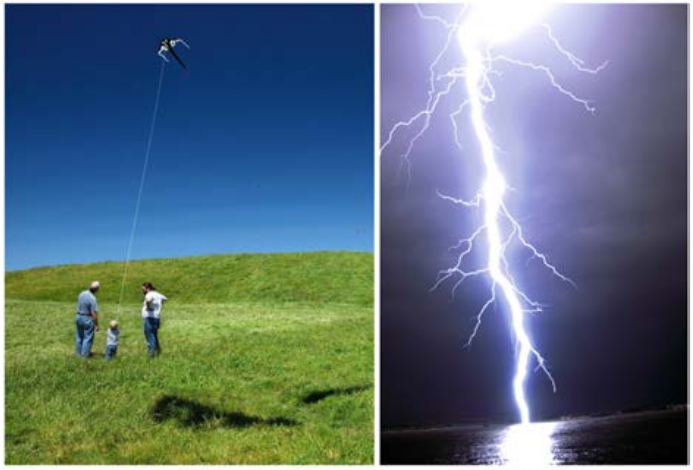
\includegraphics[width=0.5\textwidth]{figures/lightning.png}
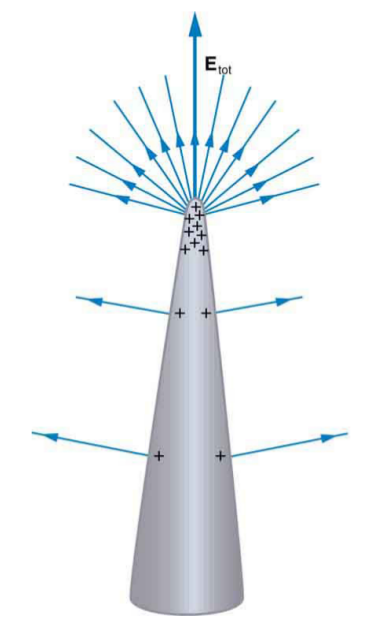
\includegraphics[width=0.25\textwidth]{figures/lightning2.png} \\
Last time...we heard some thunder!
\end{frame}

\begin{frame}{Welcome to Electromagnetism and Modern Physics!}
\centering
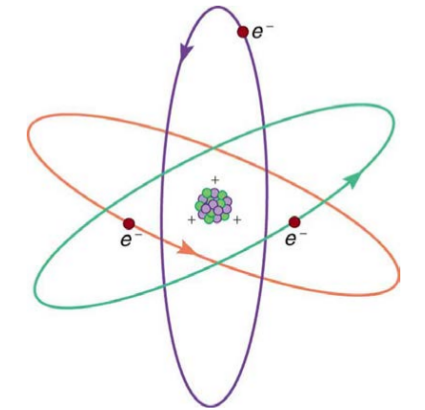
\includegraphics[width=0.7\textwidth]{figures/orbital.png}
\end{frame}

\begin{frame}{Welcome to Electromagnetism and Modern Physics!}
\centering

\includegraphics[width=0.7\textwidth]{figures/manhattan.jpg}
\end{frame}

\begin{frame}{Welcome to Electromagnetism and Modern Physics!}
\centering

\includegraphics[width=0.7\textwidth]{figures/manhattan2.jpg}
\end{frame}

\begin{frame}{Unit 1 Summary}
\textbf{Reading: Chapters 18 and 19}
\begin{enumerate}
\item Charge, mass, the Coulomb force, and the gravitational force
\item Force fields
\item Electric potential and capacitance
\end{enumerate}
\end{frame}

\begin{frame}{JITT 1.1}
A potential course: \textbf{Physics of the Five Senses}
\begin{figure}
\centering
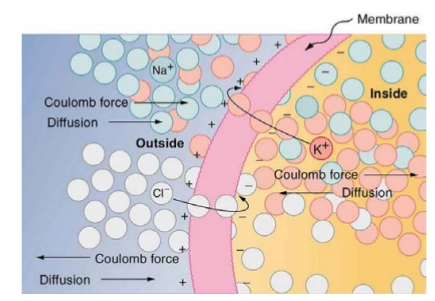
\includegraphics[width=0.6\textwidth]{figures/membrane.png}
\caption{\label{fig:membrane} The cell membrane creates a voltage.}
\end{figure}
\end{frame}

\section{Charge, Conductors and Insulators}

\begin{frame}{Charge, Conductors and Insulators}
\small
Charge the following intrinsic properties: \\ \vspace{0.25cm}
\begin{enumerate}
\item Charge is conserved globally (charge cannot be created nor destroyed).  Mass has the same property.
\item Charge is conserved locally (if we pull charge out of the system, charge will flow into the system).
\item Charge is quantized, with an electron (for example) having the fundamental negative unit, and a proton (for example) having the fundamental positive unit.
\item The laws of physics are the same for positive and negative charges.
\item The two kinds of charge emit fields that attract each other; fields emitted by charges of the same type repel such charges.
\end{enumerate}
\end{frame}

\begin{frame}{Charge, Conductors and Insulators}
\textbf{Benjamin Franklin and the Leyden Jar}.  (Good paper topic).
\begin{figure}
\centering
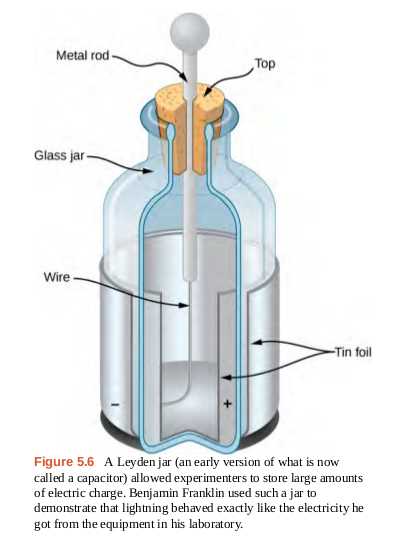
\includegraphics[width=0.3\textwidth]{figures/leyden.png}
\caption{\label{fig:leyden} A Leyden jar was an early version of a capacitor.  Benjamin Franklin guessed that one type of charge moves and another remains stationary, explaining several behaviors of charged objects.}
\end{figure}
\end{frame}

\begin{frame}{Charge, Conductors and Insulators}
The rest of the properties of charge are connected to the development of the structure of the atom, and we will return to this topic at the end of the semeter.
\begin{figure}
\centering
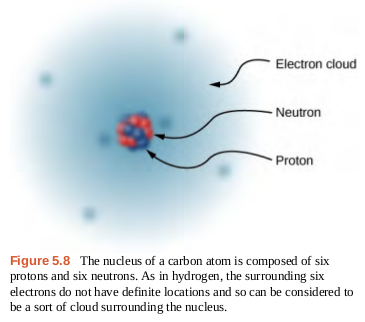
\includegraphics[width=0.5\textwidth]{figures/atom.png}
\caption{\label{fig:atom} A sketch of our current atomic paradigm.}
\end{figure}
\end{frame}

\begin{frame}{Charge, Conductors and Insulators}
Suppose an ion is composed of six protons, eight neutrons, and five electrons.  What is the net charge?
\begin{itemize}
\item A: +1
\item B: 0
\item C: -1
\item D: -2
\end{itemize}
\end{frame}

\begin{frame}{Charge, Conductors and Insulators}
An insulator with a positive charge is held next to a \textit{conductor} (an object in which charge can move around freely).  Which of the following is true?
\begin{itemize}
\item A: The charges in the conductor all remain in place because charge is conserved.
\item B: The negative charges in the conductor move toward the positive charges in the rod.
\item C: The positive charges remain in place but the negative charges move away from the rod.
\item D: The positive charges move toward the rod and the negative charges remain in place.
\end{itemize}
\end{frame}

\begin{frame}{Charge, Conductors and Insulators}
An \textit{insulator} with a net positive charge is held next to an \textit{insulator} with a net negative charge.  Which of the following is true?
\begin{itemize}
\item A: The charges in the conductor all remain in place, and the force is attractive.
\item B: The charges in the conductor all move around until the force is attractive.
\item C: The charges in the conductor all remain in place, and the force is repellent.
\item D: The charges in the conductor all move around until the force is repellent.
\end{itemize}
\end{frame}

\begin{frame}{Coulomb’s Law and Electric Fields}
The boundary conditions of problems can vary depending on the materials involved: \\ \vspace{0.5cm}
\textbf{Insulator}: A material in which there are no free charges available to conduct electricity.  Charges may be fixed in position within an insulator. \\
\textbf{Conductor}: A material in which there are free charges available to conduct electricity.  Charges may not be fixed in position within a conductor. \\
\textbf{Semi-conductor}: A material in which there are free charges available to conduct electricity if certain requirements are met.
\end{frame}

\section{Activity: PhET Simulation of Charges and Fields}

\begin{frame}{Activity: PhET Charges and Fields}
At your tables, go to the following URL: \\ \vspace{0.2cm}
\url{https://phet.colorado.edu/en/simulation/charges-and-fields} \\ \vspace{0.2cm}
Click on the java app to get it running.  Notice the following:
\begin{enumerate}
\item This is a 2D coordinate space, and you can activate the grid lines at right, by clicking \textit{grid.}
\item Clicking \textit{values} gives you the measurement scale.
\item Click \textit{electric field}, or make sure it is activated.
\item Verify the length scale with the \textbf{ruler tool}, shaped like a tape measure.  It can be dragged from the box at right.
\end{enumerate}
\end{frame}

\begin{frame}{Activity: PhET Charges and Fields}
\small
\url{https://phet.colorado.edu/en/simulation/charges-and-fields} \\ \vspace{0.2cm}
\textbf{Click and drag a positive charge into the 2D coordinate system.  This is analagous to charging an insulator.}
\begin{enumerate}
\item Drag the yellow tool at the bottom into the space, and use it to measure the field strength.  Notice the units are in V/m and m.
\item Copy to excel the field strength (E) versus distance (r).  Use 25 cm distance increments, and record 15 data points in two columns.
\item In a third column, compute $r^2 E$.
\end{enumerate}
\end{frame}

\begin{frame}{Activity: PhET Charges and Fields}
\small
\url{https://phet.colorado.edu/en/simulation/charges-and-fields} \\ \vspace{0.2cm}
\textbf{Click and drag a positive charge into the 2D coordinate system.  This is analagous to charging an insulator.}
\begin{enumerate}
\item Plot $r^2 E$ vs. $r$.  Do you observe a flat line?  What are some sources of error that contribute to the uncertainty in the slope?
\item Repeat this same exercise, but instead of measuring field strength versus \textit{distance}, measure it in one location, versus \textit{charge.} Take 15 data points in two columns and plot the results in Excel.  What is the slope of the line?  Notice the units of charge are nC.
\end{enumerate}
\textbf{Example data:} See Moodle for sample data drawn from this PhET.
\end{frame}

\begin{frame}{Charge, Conductors and Insulators}
\centering
\textbf{\alert{Charge: the constant of proportionality between the strength of a \textit{field} and the force a field exerts on an \textit{object}.}} \\
\hrulefill
\small
\begin{columns}[T]
\begin{column}{0.5\textwidth}
\alert{Gravity}
\begin{enumerate}
\item Force: $\vec{F} = G \frac{m M}{r^2} \hat{r}$
\item Parameters: $r$ is absolute distance between two objects with masses $m$ and $M$, and the direction is $\hat{r}$
\item \textit{Charge} of one object: $m$
\item \textit{Field felt by that object}: $\vec{G} = G \frac{M}{r^2} \hat{r}$
\item $\vec{F} = m \vec{G}$
\end{enumerate}
\end{column}
\begin{column}{0.5\textwidth}
\alert{Electricity}
\begin{enumerate}
\item Force: $\vec{F} = k \frac{q Q}{r^2} \hat{r}$
\item Parameters: $r$ is absolute distance between two objects with electric charges $q$ and $Q$, and the direction is $\hat{r}$
\item \textit{Charge} of one object: $q$
\item \textit{Field felt by that object}: $\vec{E} = G \frac{Q}{r^2} \hat{r}$
\item $\vec{F} = q \vec{E}$
\end{enumerate}
\end{column}
\end{columns}
\end{frame}

\begin{frame}{Charge, Conductors and Insulators}
\centering
\textbf{\alert{Charge: the constant of proportionality between the strength of a \textit{field} and the force a field exerts on an \textit{object}.}} \\
\hrulefill \\
\small
In the field paradigm, objects with charges \textit{emanate} fields, causing other objects with charge to experience force. \\
\hrulefill \\
\begin{columns}[T]
\begin{column}{0.5\textwidth}
\alert{Gravity} \\
How many \textit{types of charge}, or how many charges, exist under the force of gravity? \\
\textbf{One.} We call it mass.
\end{column}
\begin{column}{0.5\textwidth}
\alert{Electricity} \\
How many \textit{types of charge}, or how many charges, exist under the force of electricity? \\
\textbf{Two.} We call one positive, and one negative.
\end{column}
\end{columns}
\end{frame}

\begin{frame}{Charge, Conductors and Insulators}
\centering
\textbf{\alert{Charge: the constant of proportionality between the strength of a \textit{field} and the force a field exerts on an \textit{object}.}} \\
\hrulefill \\
\small
In the field paradigm, objects with charges \textit{emanate} fields, causing other objects with charge to experience force. \\
\hrulefill \\
In the field paradigm, gravity has one charge (mass), and electricity has two charges (positive and negative). \\
\hrulefill \\
\textbf{There is one fundamental fact that is puzzling.} What about Newton's 2nd law?  Acceleration is not a field, it is a kinematic function.
\begin{equation}
\vec{F}_{\rm net} = m \vec{a}
\end{equation}
Aparently there are \textit{two kinds of mass}: \textbf{inertial} and \textbf{gravitational}.  
\end{frame}

\begin{frame}{Charge, Conductors and Insulators}
\small
\textit{Equivalence principle:} \\ \hrulefill \\
There are \textit{two kinds of mass}: \textbf{inertial} and \textbf{gravitational}, with \textbf{equal value} for a given object. \\ \vspace{0.5cm}
\url{https://en.wikipedia.org/wiki/Equivalence_principle} \\
\hrulefill \\
There is no similar principle for charge.  If the electric force on a charged object is calculated, that force must still be inserted into \textbf{Newton's 2nd Law} to obtain the acceleration, and the inertial mass must be known.
\end{frame}

\section{Coulomb’s Law and Electric Fields}

\begin{frame}{Coulomb’s Law and Electric Fields}
\textbf{Coulomb's Law} describes the force between charges. \\ \vspace{0.5cm}
\begin{tcolorbox}[colback=white,colframe=black!100!black,title=Coulomb's Law]
\alert{The electric force, or \textbf{Coulomb force}, between two electrically charged systems with charges $q_{\rm 1}$ and $q_{\rm 2}$ separated by a distance $r$ is
\begin{equation}
\vec{F}_{\rm C} = \frac{1}{4\pi\epsilon_{\rm 0}} \frac{q_{\rm 1} q_{\rm 2}}{r^2} \hat{r} \label{eq:C}
\end{equation}
In Eq. \ref{eq:C}, $\hat{r} = \vec{r}/|\vec{r}|$, and $\epsilon_{\rm 0} = 8.85418782\times 10^{-12} N^{-1} m^{-2} C^2$, called the \textit{perimittivity of free space.}}
\end{tcolorbox}
\end{frame}

\begin{frame}{Coulomb’s Law and Electric Fields}
\begin{tcolorbox}[colback=white,colframe=black!100!black,title=Coulomb Field]
\alert{The electric field corresponding to Eq. \ref{eq:C}, experienced by a charge $q$ and generated by a charge $Q$ is 
\begin{equation}
\vec{E}_{\rm C} = \frac{1}{4\pi\epsilon_{\rm 0}} \frac{Q}{r^2} \hat{r} \label{eq:Cf}
\end{equation}
In Eq. \ref{eq:Cf}, $r$ remains the separation between $q$ and $Q$.}
\end{tcolorbox}
Thus we have: $\vec{F}_{\rm C} = q \vec{E}_{\rm C}$. \\ \vspace{0.5cm}
The SI Unit of charge is the Coulomb, which is equal to the amount of charge in a "current" of 1 amp for 1 second (more on this later).  \textbf{The charge of an electron is $1.6\times 10^{-19}$ Coulombs, or C.}
\end{frame}

\begin{frame}{Coulomb’s Law and Electric Fields}
Suppose a charge $+q$ experiences the Coulomb field of another charge of $-q$, separated by a distance $r$.  Which of the following is true?
\begin{itemize}
\item A: The charge $+q$ accelerates the $-q$ charge only.
\item B: The charge $-q$ accelerates the $+q$ charge only.
\item C: No charges move; the force on one is equal to the force on the other.
\item D: Both charges move, and the force on one is equal to the force on the other.
\end{itemize}
\end{frame}

\begin{frame}{Coulomb’s Law and Electric Fields}
The answer to the previous problem involves Newton's Third Law.
\begin{figure}
\centering
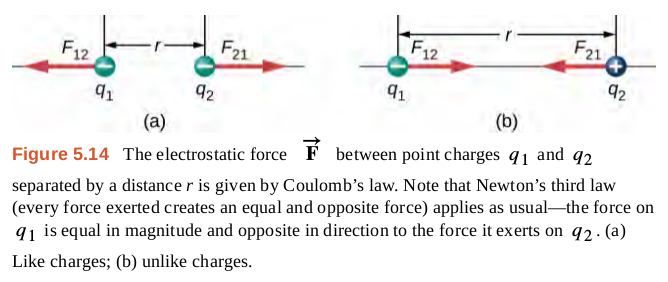
\includegraphics[width=0.9\textwidth]{figures/third.png}
\caption{\label{fig:third} Newton's Third Law still applies.}
\end{figure}
\end{frame}

\begin{frame}{Coulomb’s Law and Electric Fields}
\small
\begin{columns}[T]
\begin{column}{0.5\textwidth}
What is the angle of the E-field at point (1,1) in Fig. \ref{fig:netfield2} at right?
\begin{itemize}
\item A: 0 deg
\item B: 45 deg
\item C: 90 deg
\item D: 135 deg
\end{itemize}
What is the fastest way to solve this problem?
\begin{itemize}
\item A: Blind luck
\item B: Do the algebra
\item C: Symmetry
\item D: Numerical estimation
\end{itemize}
\end{column}
\begin{column}{0.5\textwidth}
\begin{figure}
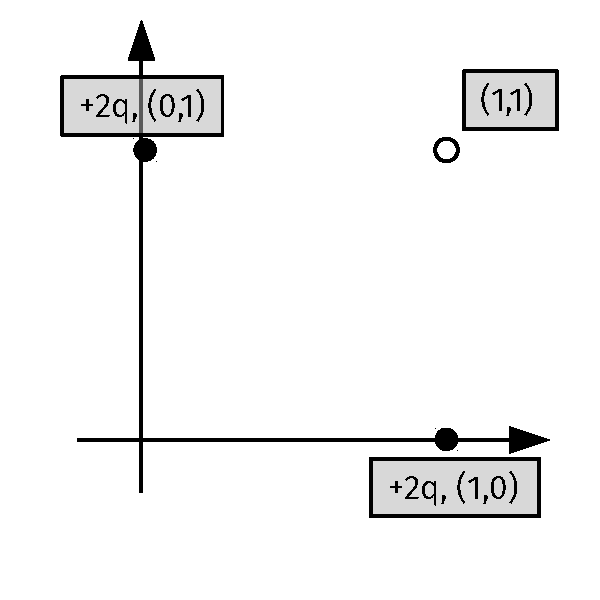
\includegraphics[width=\textwidth]{figures/NetField2.pdf}
\caption{\label{fig:netfield2} Two charges create a field for a hypothetical \textit{test charge}.}
\end{figure}
\end{column}
\end{columns}
\end{frame}

\begin{frame}{Coulomb’s Law and Electric Fields}
\small
\begin{columns}[T]
\begin{column}{0.5\textwidth}
Which of the following is true of the E-field at point (1,1) in Fig. \ref{fig:netfield3} at right?
\begin{itemize}
\item A: The angle with respect to the x-axis is 45 degrees
\item B: The angle with respect to the x-axis is greater than 45 degrees
\item C: The angle with respect to the x-axis is less than 45 degrees
\item D: The angle with respect to the x-axis is 90 degrees
\end{itemize}
\end{column}
\begin{column}{0.5\textwidth}
\begin{figure}
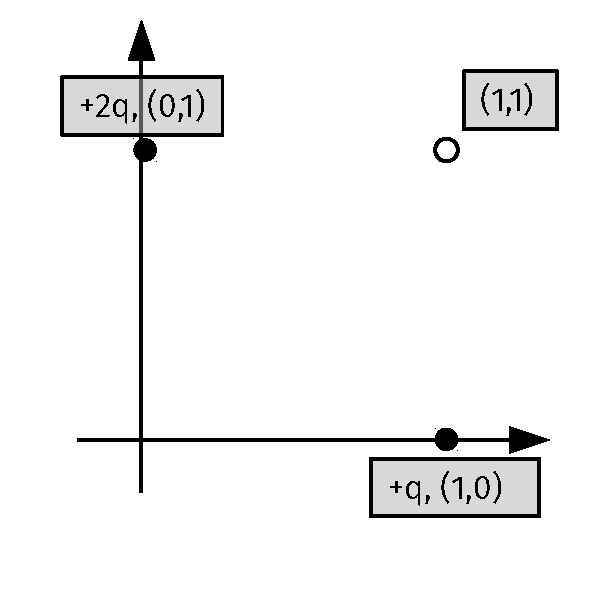
\includegraphics[width=\textwidth]{figures/NetField3.pdf}
\caption{\label{fig:netfield3} Two charges create a field for a hypothetical \textit{test charge}.}
\end{figure}
\end{column}
\end{columns}
\end{frame}

\begin{frame}{Coulomb’s Law and Electric Fields}
\small
\begin{columns}[T]
\begin{column}{0.5\textwidth}
\textbf{Table exercise:} Calculate $\vec{E}_{\rm C,Net}(P)$, if $P = (1,1)$. \\ \vspace{0.5cm}
\textbf{Table exercise:} Calculate $\vec{E}_{\rm C,Net}(P)$, if $P = (-1,-1)$. \\ \vspace{0.5cm}
\textbf{Group discussion:} What does it mean if $P = (1,0)$? \\ \vspace{0.5cm}
\end{column}
\begin{column}{0.5\textwidth}
\begin{figure}
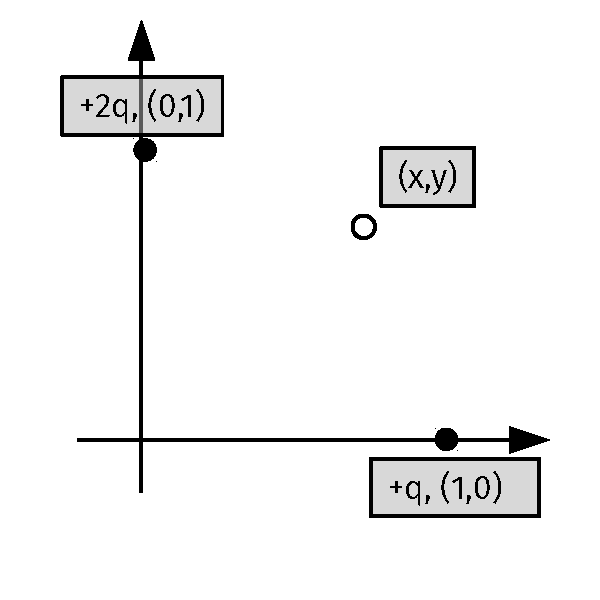
\includegraphics[width=\textwidth]{figures/NetField4.pdf}
\caption{\label{fig:netfield4} Two charges create a field for a hypothetical \textit{test charge}.}
\end{figure}
\end{column}
\end{columns}
\end{frame}

\begin{frame}{Coulomb’s Law and Electric Fields}
Have you noticed that the Coulomb force does not depend on kinematic variables like velocity, or have any dissipative effect?  Perhaps it is \alert{\textbf{conservative}}.  In your own words at your table, discuss the meaning of a conservative force. \\ \vspace{0.5cm}
\small
If a force $F$ is conservative, what is the relationship between $F$ and the potential energy, $U$?
\begin{itemize}
\item A: $F$ is proportional to the kinetic energy, which is related to $U$.
\item B: $F$ is proportional to the change in $-U$
\item C: Work done on a system going against $F$ is path independent, so $U$ is the same if the system's path is closed
\item D: B and C
\end{itemize}
\end{frame}

\begin{frame}{Coulomb’s Law and Electric Fields}
If a force is conservative, it is true that
\begin{equation}
F = -\frac{\Delta U}{\Delta x}
\end{equation}
In kinematics, $U$ is the potential energy.  In electrostatics, we write it as a \textit{voltage.}
\begin{equation}
E = -\frac{\Delta V}{\Delta x}
\end{equation}
\begin{enumerate}
\item Hill analogy.
\item Voltage on the PhET simulation.
\end{enumerate}
\end{frame}

\begin{frame}{Coulomb’s Law and Electric Fields}
The forces of $N$ fixed charges on a test charge $Q$ create a net force, where the individual forces simply add like vectors.  This is known as the \textbf{superposition principle}.
\begin{align}
\vec{F}_{\rm C,Net} &= \frac{1}{4\pi\epsilon_{\rm 0}} Q \sum_{i = 1}^N \frac{q_i}{r_i^2}\hat{r}_i = Q \vec{E}_{\rm C,Net} \\
\vec{E}_{\rm C,Net} &= \frac{1}{4\pi\epsilon_{\rm 0}} \sum_{i = 1}^N \frac{q_i}{r_i^2}\hat{r}_i
\end{align}
\end{frame}

\begin{frame}{Coulomb’s Law and Electric Fields}
For the expressions of fields built from the superposition principle, let's adopt a notation:
\begin{equation}
\vec{E}_{\rm C,Net}(P) = \frac{1}{4\pi\epsilon_{\rm 0}} \sum_{i = 1}^N \frac{q_i}{r_i^2}\hat{r}_i \label{eq:P}
\end{equation}
Equation \ref{eq:P} represents the field at a \textit{position} $P = P(x,y,z)$, relative to the positions $\vec{r}_i$ of the source charges.
\end{frame}

\begin{frame}{Coulomb’s Law and Electric Fields}
\small
\begin{columns}[T]
\begin{column}{0.5\textwidth}
The following problem is an example of solving for a field analytically, and \textit{testing various limits}.  Upon taking limits results are often simple and intuitive. \\ \vspace{0.5cm}
Two charges $+q$ are on the fixed in an insulator on the x-axis.  Solve for the E-field at $P = (0,0,z)$. \\ \vspace{0.5cm}
(Professor demonstrate on board).
\begin{equation}
\vec{E}(z) = \frac{1}{4\pi\epsilon_0} \frac{2qz}{\left(z^2+\left(\frac{d}{2}\right)^2\right)^{3/2}} \hat{k}
\end{equation}
\end{column}
\begin{column}{0.5\textwidth}
\begin{figure}
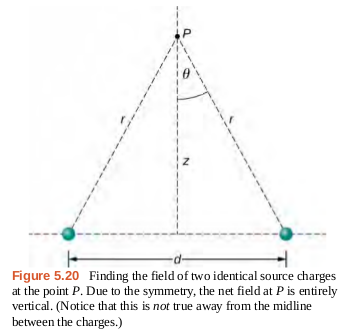
\includegraphics[width=\textwidth]{figures/twoChargesZ.png}
\caption{\label{fig:twoChargesZ} Solve for the E-field as a function of $z$, $d$, and $q$.}
\end{figure}
\end{column}
\end{columns}
\end{frame}

\begin{frame}{Coulomb’s Law and Electric Fields}
\small
\begin{columns}[T]
\begin{column}{0.5\textwidth}
Show that the general solution is
\begin{equation}
\vec{E}(z) = \frac{1}{4\pi\epsilon_0} \frac{2qz}{\left(z^2+\left(\frac{d}{2}\right)^2\right)^{3/2}} \hat{k}
\end{equation}
\textit{Take the following two limits:} \\ 1) $z \gg d$ and 2) $z=0$.  What are the results? \\ \vspace{0.5cm}
Keep these results in mind, because we are about to start drawing \textbf{vector fields,} in order to visualize the algebra.
\end{column}
\begin{column}{0.5\textwidth}
\begin{figure}
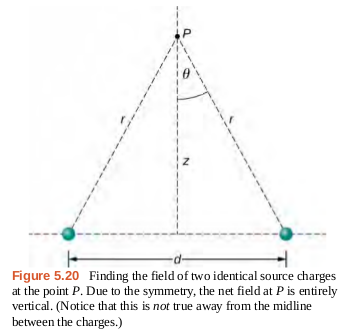
\includegraphics[width=\textwidth]{figures/twoChargesZ.png}
\caption{\label{fig:twoChargesZ2} Solve for the E-field as a function of $z$, $d$, and $q$.}
\end{figure}
\end{column}
\end{columns}
\end{frame}

\section{Activity: PhET Simulation of Charges and Fields}

\begin{frame}{Coulomb’s Law and Electric Fields}
\textbf{PhET Simulation of E-fields from Charges}: \\ \vspace{0.5cm}
\url{https://phet.colorado.edu/en/simulation/charges-and-fields}
\begin{enumerate}
\item Create the situation in the prior problem, in Fig. \ref{fig:twoChargesZ2}.
\item Use the yellow sensor object to determine the local direction of the E-field at various points along the z-axis.
\begin{itemize}
\item Do the results match the limit $z\gg d$?
\item Do the results match the limit $z = 0$, halfway between the charges?
\item Where is the field maximal?
\end{itemize}
\item Make sure you can see above and below the charges, and repeat steps 1 and 2 for negative z-values.  What do you find?
\end{enumerate}
\end{frame}

\begin{frame}{Coulomb’s Law and Electric Fields}
\small
\textbf{PhET Simulation of E-fields from Charges}: \\ \vspace{0.5cm}
Build E-fields with the following properties, by adding single charges.  Let the \textit{z-axis be upwards}, and let the \textit{x-axis be to the right.}
\begin{enumerate}
\item Build an electric field that has \textbf{reflection symmetry} across the z-axis, with at least five charges.
\item Build an electric field that has \textit{radial symmetry} about the origin, with at least six charges.
\item Build an electric field that would be the same if I rotated the picture by 90 degrees (\textbf{4-fold symmetry}) with at least four charges, some negative and some positive.
\item Build an electric field that would be the same if I rotated the picture by 45 degrees (\textbf{8-fold symmetry}) with at least eight charges, some negative and some positive.
\end{enumerate}
\end{frame}

\begin{frame}{Coulomb’s Law and Electric Fields}
When we connect the vectors in a vector field, the results are figures like Fig. \ref{fig:lines}.  Fields by convention originate from positive charges and terminate on negative ones.
\begin{figure}
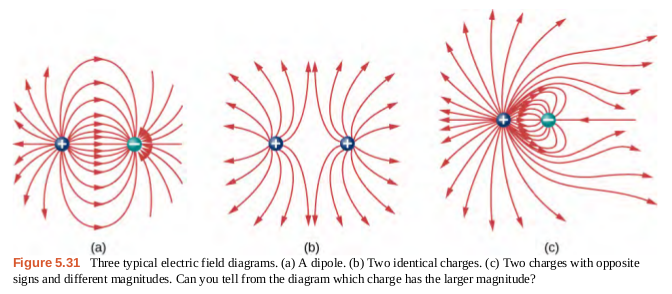
\includegraphics[width=0.8\textwidth]{figures/lines.png}
\caption{\label{fig:lines} Field-line diagrams.  The density of lines indicates electric field strength.}
\end{figure}
\end{frame}

\begin{frame}{Coulomb’s Law and Electric Fields}
\small
Different PhET simulations and programs to illustrate field lines:
\begin{enumerate}
\item \textbf{\url{http://www.flashphysics.org/electricField.html}}
\item \textit{\url{https://phet.colorado.edu/en/simulation/electric-hockey}}
\item \textit{\url{https://phet.colorado.edu/en/simulation/efield}}
\end{enumerate}
Homework bonus point: use (1) to draw the electric field of a water molecule.  Make sure it has the correct number of positive and negative charges, in the correct positions.
\end{frame}

\begin{frame}{Coulomb’s Law and Electric Fields}
\begin{figure}
\centering
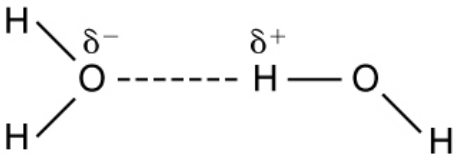
\includegraphics[width=0.6\textwidth]{figures/water.png}
\caption{\label{fig:water} Two water molecules with hydrogen bonds.}
\end{figure}
\end{frame}

\section{E-Fields of Charge Distributions}

\begin{frame}{E-Fields of Charge Distributions}
Let $k = 1/(4\pi\epsilon_0)$.
\begin{equation}
\vec{E}(P) = k \sum_{i = 1}^N \left(\frac{q_i}{r_i^2}\right) \hat{r} \label{eq:point}
\end{equation}
Imagine a charged object with a distinct shape. To obtain the E-field, all we have to do is \textit{break it into manageable pieces.}
\begin{enumerate}
\item Decide where to compute the field $(P)$.
\item Evaluate Eq. \ref{eq:point} for each little piece.
\item Add up the total using vector addition.
\item \textbf{These calculations speed up if we use symmetry!}
\end{enumerate}
\end{frame}

\begin{frame}{E-Fields of Charge Distributions}
\small
\begin{figure}
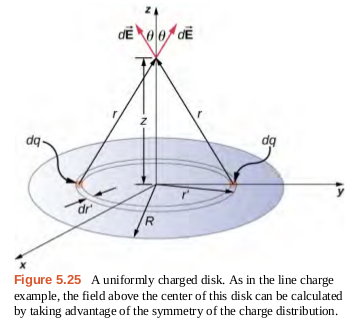
\includegraphics[width=0.4\textwidth]{figures/disk.png}
\caption{\label{fig:disk2} \textit{Continuous} distributions are solved with calculus\footnote{Imagine calculating the mass of an object, knowing the function that describes density in 3D space}.}
\end{figure}
\end{frame}

\begin{frame}{E-Fields of Charge Distributions}
\small
The result:
\begin{equation}
\boxed{
\vec{E} = k\left(2\pi\sigma - \frac{2\pi\sigma z}{\sqrt{R^2 + z^2}} \right)\hat{k}} \label{eq:disk}
\end{equation}
Which of the following is true of Eq. \ref{eq:disk}?
\begin{itemize}
\item A: Taking the limit $R \rightarrow \infty$ yields a constant field.
\item B: Taking the limit $z \rightarrow 0$ yields a constant field.
\item C: The charge distribution has radial symmetry, so the field cannot have horizontal components.
\item D: A, B, and C
\end{itemize}
\end{frame}

\begin{frame}{E-Fields of Charge Distributions}
\begin{equation}
\boxed{
\vec{E} = k\left(2\pi\sigma - \frac{2\pi\sigma z}{\sqrt{R^2 + z^2}} \right)\hat{k}} \label{eq:disk2}
\end{equation}
What happens to Eq. \ref{eq:disk2}, in the limit that $R \rightarrow \infty$?
\begin{itemize}
\item A: The field decreases to zero.
\item B: The field is constant.
\item C: The field grows increasingly positive.
\item D: The field grows increasingly negative.
\end{itemize}
\end{frame}

\begin{frame}{E-Fields of Charge Distributions}
In the limit that $R \rightarrow \infty$,
\begin{equation}
\vec{E} = 2\pi\sigma k \hat{k} = \frac{\sigma}{2\epsilon_0} \hat{k} \label{eq:disk3}
\end{equation}
Equation for the electric field of a uniform infinite disk.
\end{frame}

\begin{frame}{E-Fields of Charge Distributions}
Imagine two infinite disks with equal uniform charge distributions, some distance apart.  One has positive charge, the other negative charge.  What is the E-field between them?
\begin{itemize}
\item A: 0
\item B: $\frac{\sigma}{2\epsilon_0}$
\item C: $\frac{\sigma}{\epsilon_0}$
\item D: $\frac{\sigma}{4\epsilon_0}$
\end{itemize}
\end{frame}

\begin{frame}{E-Fields of Charge Distributions}
Imagine two infinite disks with equal uniform charge distributions, some distance apart.  Both have positive charge.  What is the E-field between them?
\begin{itemize}
\item A: 0
\item B: $\frac{\sigma}{2\epsilon_0}$
\item C: $\frac{\sigma}{\epsilon_0}$
\item D: $\frac{\sigma}{4\epsilon_0}$
\end{itemize}
\end{frame}

\begin{frame}{E-Fields of Charge Distributions}
\begin{figure}
\centering
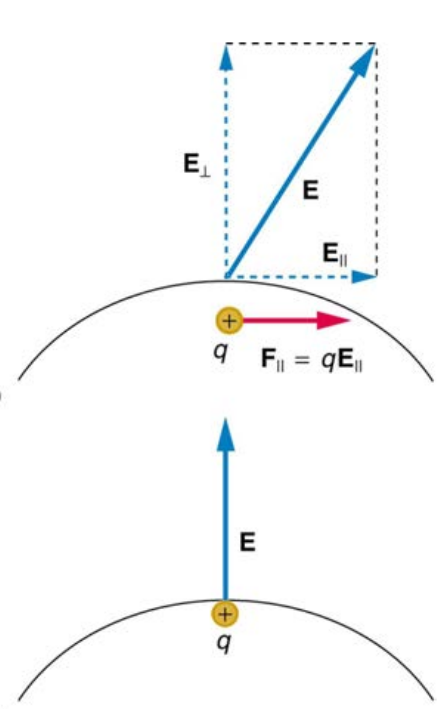
\includegraphics[width=0.3\textwidth]{figures/perp.png}
\caption{\label{fig:perp1} Free charge on a conductor distributes near the surface, and creates a perpendicular electric field.}
\end{figure}
\end{frame}

\begin{frame}{E-Fields of Charge Distributions}
\begin{figure}
\centering
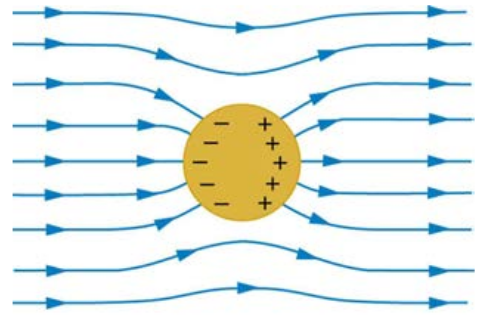
\includegraphics[width=0.7\textwidth]{figures/perp2.png}
\caption{\label{fig:perp2} An external electric field passing over a conductor.}
\end{figure}
\end{frame}

\section{Applications of Electrostatic Charging}

\begin{frame}{Applications of Electrostatic Charging}
\begin{figure}
\centering
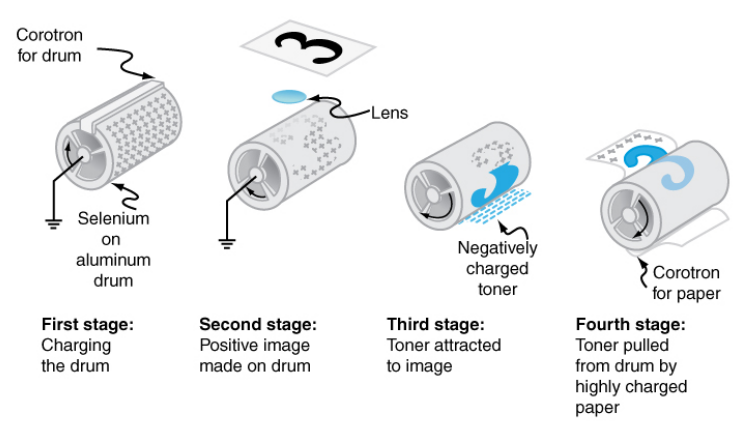
\includegraphics[width=0.7\textwidth]{figures/app1.png}
\caption{\label{fig:app1} A toner-based printer uses negatively charged toner and positively charged drums to pull toner onto the page.}
\end{figure}
\end{frame}

\begin{frame}{Applications of Electrostatic Charging}
\begin{figure}
\centering
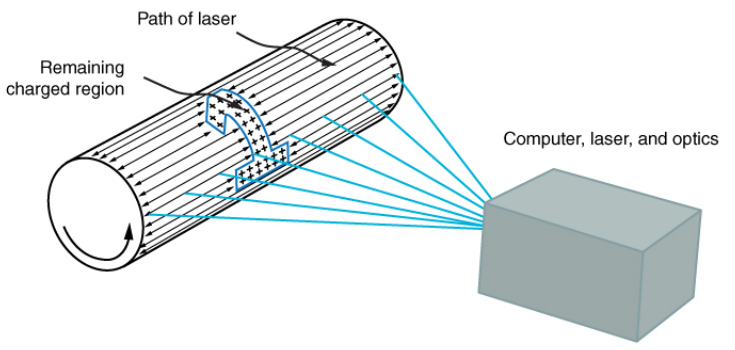
\includegraphics[width=0.7\textwidth]{figures/app2.png}
\caption{\label{fig:app2} A laser printer uses light that only darkens charged parts of the page.  This is called the xerographic process.}
\end{figure}
\end{frame}

\begin{frame}{Applications of Electrostatic Charging}
\begin{figure}
\centering
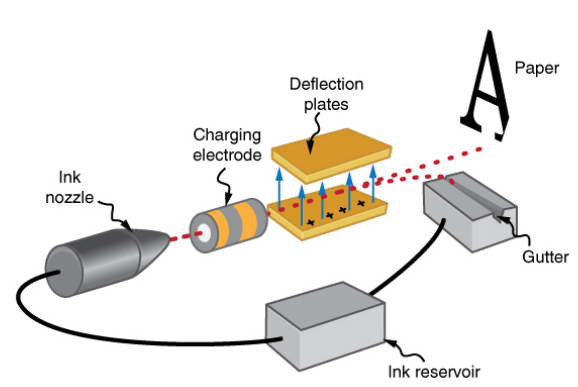
\includegraphics[width=0.7\textwidth]{figures/app3.png}
\caption{\label{fig:app3} An inkjet printer deflects charged ink with charged plates as it lands on the paper.}
\end{figure}
\end{frame}

\begin{frame}{Applications of Electrostatic Charging}
\begin{figure}
\centering
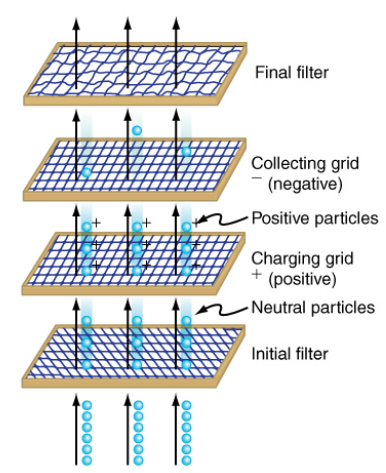
\includegraphics[width=0.4\textwidth]{figures/app4.png}
\caption{\label{fig:app4} An electromagnetic precipitator cleans air flow of particles that can be charged.}
\end{figure}
\end{frame}

\section{Electric Potential, Potential Energy}

\begin{frame}{Electric Potential, Potential Energy}
Recall that the \textit{change in potential energy} is force:
\begin{equation}
F = -\frac{\Delta U}{\Delta x}
\end{equation}
\begin{itemize}
\item The units of $U$: Joules = Newtons per meter
\item The units of $x$: meters
\item The ratio: Newtons
\end{itemize}
\end{frame}

\begin{frame}{Electric Potential, Potential Energy}
An object of mass $m$ is a height $h$ above the ground, in Earth's gravity field.  What is the \textit{potential} energy of the object?
\begin{itemize}
\item A: $U = \frac{1}{2}mv^2$ ($v$ is the velocity)
\item B: $U = \frac{1}{2}mv^2 + mgh$ ($v$ is the velocity)
\item C: $U = mgh$
\item D: $U$ is zero, because the object is at rest.
\end{itemize}
\end{frame}

\begin{frame}{Electric Potential, Potential Energy}
What is the expression for the force of gravity, if $\Delta U = mgh$, and $\Delta x = h$?
\begin{itemize}
\item A: $mg$
\item B: $-mg$
\item C: $g$
\item D: $-g$
\end{itemize}
\end{frame}

\begin{frame}{Electric Potential, Potential Energy}
\small
If the potential energy is a function of displacement, $U = U(\vec{x})$, it may be called a potential energy \textit{surface}.
\begin{figure}
\centering
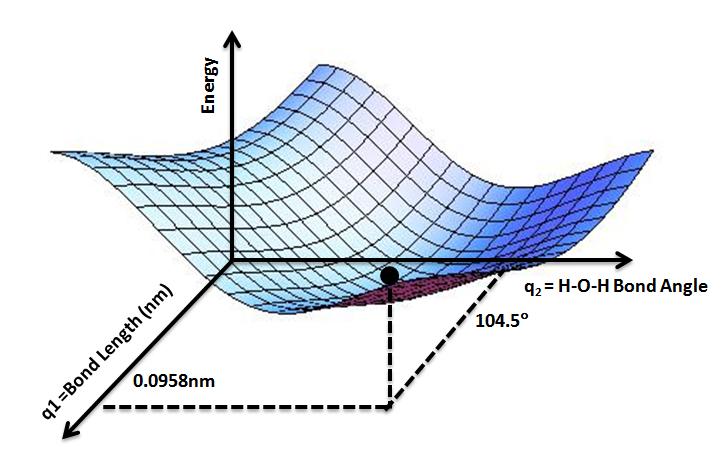
\includegraphics[width=0.5\textwidth]{figures/potential.png}
\caption{\label{fig:potential} An example of a potential energy surface.}
\end{figure}
\end{frame}

\begin{frame}{Electric Potential, Potential Energy}
\small
Considering \textit{Newton's Second Law}, however, if $F = m a$ then $m a = -\frac{\Delta U}{\Delta x}$, and
\begin{equation}
a = -\frac{1}{m}\frac{\Delta U}{\Delta x}
\end{equation}
\begin{figure}
\centering
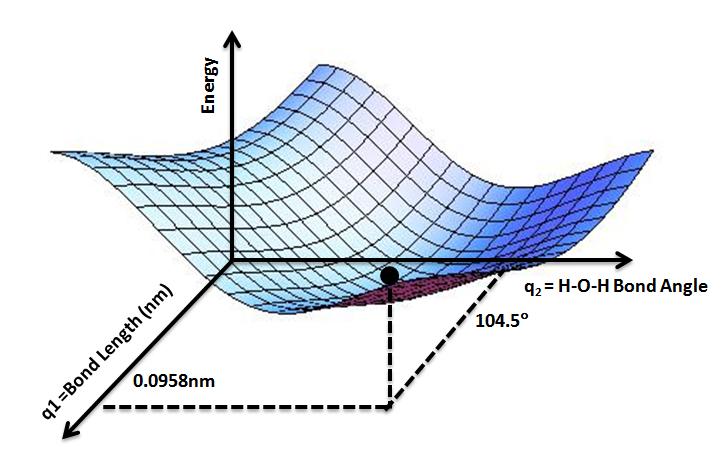
\includegraphics[width=0.5\textwidth]{figures/potential.png}
\caption{\label{fig:potential2} \small A potential energy surface.}
\end{figure}
\end{frame}

\begin{frame}{Electric Potential, Potential Energy}
\small
Let's just scale the z-axis by the mass of the system:
\begin{align}
a &= -\frac{1}{m}\frac{\Delta U}{\Delta x} \\
\Delta V &= \frac{\Delta U}{m} \\
a &= -\frac{\Delta V}{\Delta x}
\end{align}
Instead of calling $\Delta V$ the potential energy, let's just call it \textit{the potential.}  Recall that if the force is a vector field, then acceleration is a vector field as well (the object has a given acceleration vector for all points in the space).
\end{frame}

\begin{frame}{Electric Potential, Potential Energy}
\begin{columns}[T]
\begin{column}{0.5\textwidth}
\alert{Newtonian mechanics} \\ \hrulefill
\begin{align}
F &= ma \\
a &= -\frac{\Delta V}{\Delta x}
\end{align}
\end{column}
\begin{column}{0.5\textwidth}
\alert{Electrostatics} \\ \hrulefill
\begin{align}
F &= qE \\
E &= -\frac{\Delta V}{\Delta x} \label{eq:volt}
\end{align}
\end{column}
\end{columns} \vspace{1cm}
In Eq. \ref{eq:volt}, we refer to $\Delta V$ as \textbf{voltage.}
\end{frame}

\begin{frame}{Electric Potential, Potential Energy}
\small
\textbf{Voltage} is \textit{potential energy per unit charge.} \\ \vspace{0.5cm}
\url{https://phet.colorado.edu/en/simulation/charges-and-fields} \\
\begin{enumerate}
\item Place a positive charge at left, and measure the voltage with the blue tool.
\item Voltage is like potential energy per unit charge, so it should be a \textit{number}, not a \textit{vector.}
\item Measure the voltage in 25 cm increments for 15 data points, and copy the data to Excel.  One column should be the distance $r$ in meters, and the other column should be the voltage $V$ in \textbf{Volts.}
\item Plot the data in Excel, and fit a \textit{power-law} trendline to the data.  What do you notice?
\item Plot $rV$ vs. $r$.  What do you notice?
\end{enumerate}
\end{frame}

\begin{frame}{Electric Potential, Potential Energy}
Same PhET simulation:
\begin{enumerate}
\item Measure the voltage from the same charge and tool position (fixed $r$), but vary the \textit{amount of charge.}
\item Take 15 measurements, adding a positive red charge each time.
\item Plot the voltage in \textbf{Volts} vs. the charge in nano-Coulombs (nC).  What do you notice?
\end{enumerate}
\end{frame}

\begin{frame}{Electric Potential, Potential Energy}
Voltage due to a point charge:
\begin{equation}
\boxed{
V = \pm \frac{1}{4\pi \epsilon_0} \frac{q}{r}} \label{eq:volt2}
\end{equation}
Equation \ref{eq:volt2} follows from the form of the electric field of a point charge, and $E = -\Delta V/\Delta x$ (derivative, calculus).
\end{frame}

\begin{frame}{Electric Potential, Potential Energy}
Voltage is an example of a \textbf{scalar field}, whereas the electric field is an example of a \textbf{vector field.}  Recall the result for the electric field of a large plane of charge, with charge $\sigma$ per unit area:
\begin{equation}
\vec{E} = \frac{\sigma}{2\epsilon_0} \hat{k}
\end{equation}
What should the voltage be, if the field is constant?\footnote{\textit{Hint: E-field is like the slope of voltage, in the same way force is the slope of potential energy.}}
\end{frame}

\begin{frame}{Electric Potential, Potential Energy}
\begin{figure}
\centering
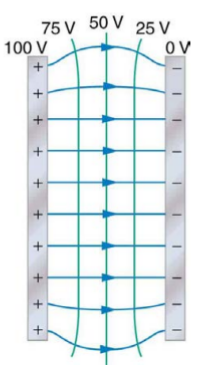
\includegraphics[width=0.25\textwidth]{figures/plates.png}
\caption{\label{fig:plates} Parallel plates of charge, electric field, and potential.  Notice the linear decrease in voltage.  Did you see this in the PhET?}
\end{figure}
\end{frame}

\begin{frame}{Electric Potential, Potential Energy}
\textit{Two parallel plates, opposite charge}:
\begin{equation}
V = -\frac{\sigma}{\epsilon_0}z + C
\end{equation}
With the boundary condition that $V = V_0$ when $z = 0$, we have
\begin{equation}
V(z) - V_0 = -\frac{\sigma}{\epsilon_0}z
\end{equation}
Let $\Delta V(z) = V(z) - V_0$, and $\Delta z = z$:
\begin{equation}
-\frac{\Delta V}{\Delta z} = \frac{\sigma}{\epsilon_0} =  E
\end{equation}
\end{frame}

\section{Voltage, Potential Energy, and Work}

\begin{frame}{Voltage, Potential Energy, and Work}
\small
What follows is a series of memorizable equations and mental images comparing voltage to gravitational potential energy.  This analogy runs deep because the Coulomb force is conservative.
\begin{figure}
\centering
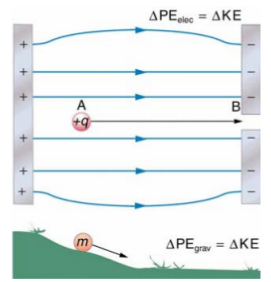
\includegraphics[width=0.45\textwidth]{figures/hill.png}
\caption{\label{fig:hill} Remembering the connection of voltage to gravity.}
\end{figure}
\end{frame}

\begin{frame}{Voltage, Potential Energy, and Work}
Imagine trying to calculate the work done ($W = -\Delta PE$) on a charge $q$ as it moves through a complex vector field ($F = qE$, where $E$ can come from some complex charge distribution).  It's easier to take the test charge $q$ out of it, and think of just the potential surface as a surface, rather than proportional to $qE$ times the path.
\begin{equation}
V = \frac{PE}{q}
\end{equation}
This makes the unit of one Volt equal to one Joule per Coulomb. (1 V = 1 J/C).  The volt reminds us of all those times the \textit{mass drops out} of the problems when we are not concerned with how many Newtons, just where things are going.
\end{frame}

\begin{frame}{Voltage, Potential Energy, and Work}
For potential energy calculations involving gravity, \textbf{we} get to decide the location of ``zero energy,'' and we're only interested in \textit{changes} in potential energy.
\begin{equation}
\Delta V = V_{\rm B} - V_{\rm A} = \frac{\Delta PE}{q}
\end{equation}
Where is the most logical place to put the voltage zero point?
\end{frame}

\begin{frame}{Voltage, Potential Energy, and Work}
\begin{figure}
\centering
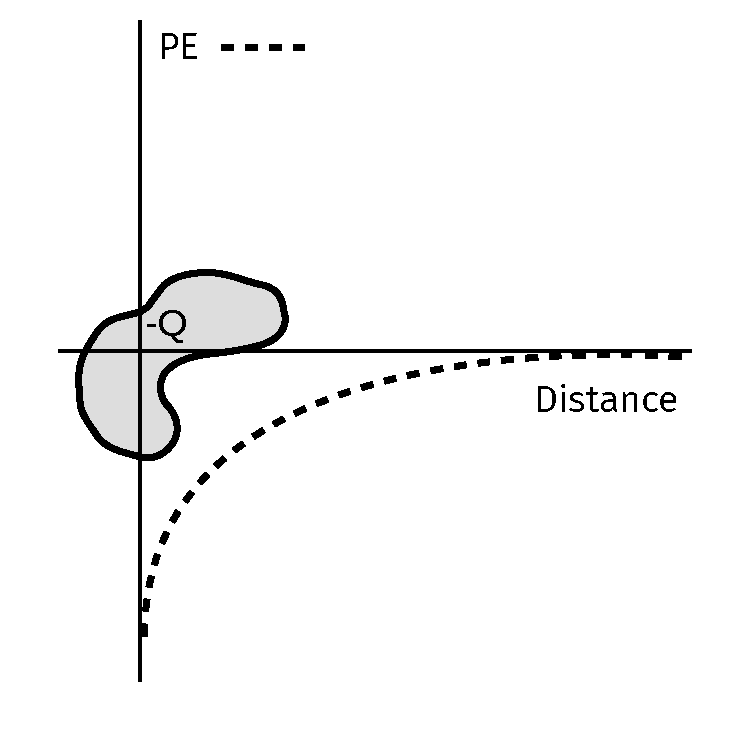
\includegraphics[width=0.6\textwidth]{figures/PE.pdf}
\caption{\label{fig:PE} Where should we place the zero point of potential energy here?  Which way do positive charges fall?  Which way do negative charges fall?}
\end{figure}
\end{frame}

\begin{frame}{Voltage, Potential Energy, and Work}
\begin{figure}
\centering
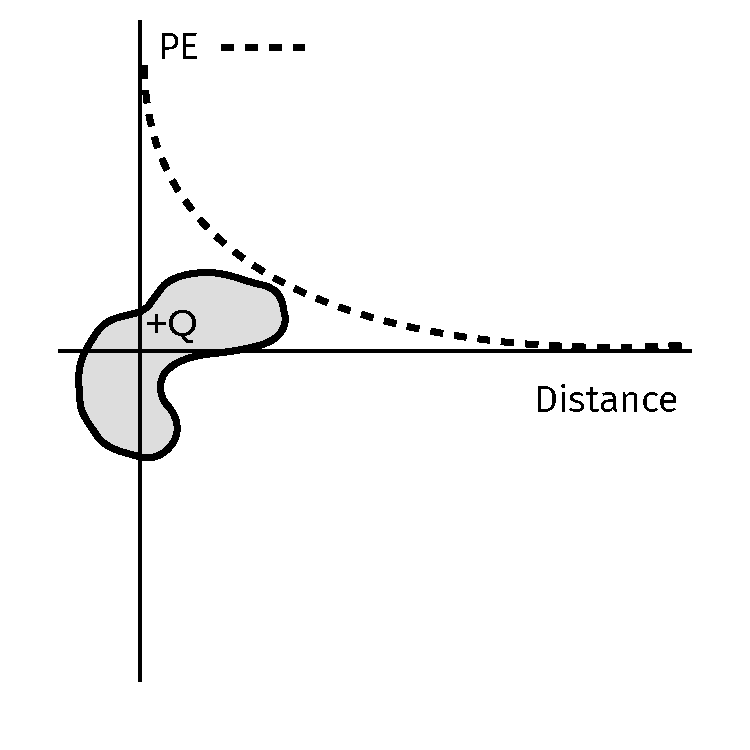
\includegraphics[width=0.6\textwidth]{figures/PE2.pdf}
\caption{\label{fig:PE2} Where should we place the zero point of potential energy here?  Which way do positive charges fall?  Which way do negative charges fall?}
\end{figure}
\end{frame}

\begin{frame}{Voltage, Potential Energy, and Work}
Suppose you have a 12.0 V motorcycle battery that can move 5000 C of charge, and a 12.0 V car battery that can move 60,000 C of charge. How much energy does each deliver?
\begin{itemize}
\item A: 60 kJ and 720 kJ, respectively
\item B: 600 kJ and 7200 kJ, respectively
\item C: 6 kJ and 72 kJ, respectively
\item D: 0.6 kJ and 7.2 kJ, respectively
\end{itemize}
\end{frame}

\begin{frame}{Voltage, Potential Energy, and Work}
\begin{figure}
\centering
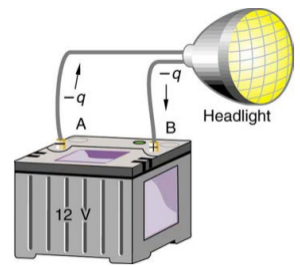
\includegraphics[width=0.6\textwidth]{figures/headlight.png}
\caption{\label{fig:headlight.png} Here is a battery circuit that has a potential difference of 12 V.  Where would you put the zero point?}
\end{figure}
\end{frame}

\begin{frame}{Voltage, Potential Energy, and Work}
Consider the battery headlight circuit.  The car batter has 60,000 C stored, with $\Delta V = 12.0$ V.  The headlight requires 30 W of power.  We know how much energy is in the battery, so how long can the headlight run?
\begin{itemize}
\item A: About 1 hour
\item B: About 2 hours
\item C: About 7 hours
\item D: About 9 hours
\end{itemize}
\end{frame}

\begin{frame}{Voltage, Potential Energy, and Work}
\textbf{Smaller than a motorcycle battery}: Suppose an AA battery has 1.5 V, and 7200 C of charge.  How much energy is stored inside it?
\begin{itemize}
\item A: About 5 kJ
\item B: About 10 kJ
\item C: About 15 kJ
\item D: About 20 kJ
\end{itemize}
\end{frame}

\begin{frame}{Voltage, Potential Energy, and Work}
Same headlight: requires 30 W of power.  We know how much energy is in the battery, so how long can the headlight run?
\begin{itemize}
\item A: About 1 hour
\item B: About 30 minutes
\item C: About 15 minutes
\item D: About 6 minutes
\end{itemize}
\end{frame}

\begin{frame}{Voltage, Potential Energy, and Work}
\textbf{Scaling problems:} Consider two batteries.  Battery 1 has 5000 C at 12 V.  Battery 2 has the same charge but only 3/4 the energy.  What is the voltage of battery 2?
\begin{itemize}
\item A: 5 V 
\item B: 7 V
\item C: 9 V
\item D: 12 V
\end{itemize}
\end{frame}

\begin{frame}{Voltage, Potential Energy, and Work}
\textbf{Review}: recall that the potential of a point charge with charge $q$ at a distance $r$ is $V(r) = kq/r$.  Suppose a charge has 10 V at a distance of 1 cm.  What is the potential at 10 cm?
\begin{itemize}
\item A: 10 V 
\item B: 5 V
\item C: 2 V
\item D: 1 V
\end{itemize}
\textit{Where is the ``zero point'' of the voltage?}
\end{frame}

\begin{frame}{Voltage, Potential Energy, and Work}
\textbf{Group problem}: We have a solar-panel system, but it's not running our application long enough.  Suppose the battery is a 24V battery that can run a 10 W system for 24 hours.  If we add a second 24V battery with half the charge of the first, for how long can the system run? \\ \vspace{0.5cm}
\textit{When your group has the solution, draw it on the nearest whiteboard.}
\end{frame}

\begin{frame}{Voltage, Potential Energy, and Work}
\textbf{The electron-Volt, eV}: Since charge times voltage is energy, why not have a unit where it's the charge of one electron through a potential difference of one volt? \\ \vspace{0.5cm}
$q_{\rm e} \approx 1.6 \times 10^{-19}$ C, 1 eV = $1.6 \times 10^{-19}$ J. \\ \vspace{0.5cm}
This unit comes in handy!
\end{frame}

\begin{frame}{Voltage, Potential Energy, and Work}
\begin{figure}
\centering
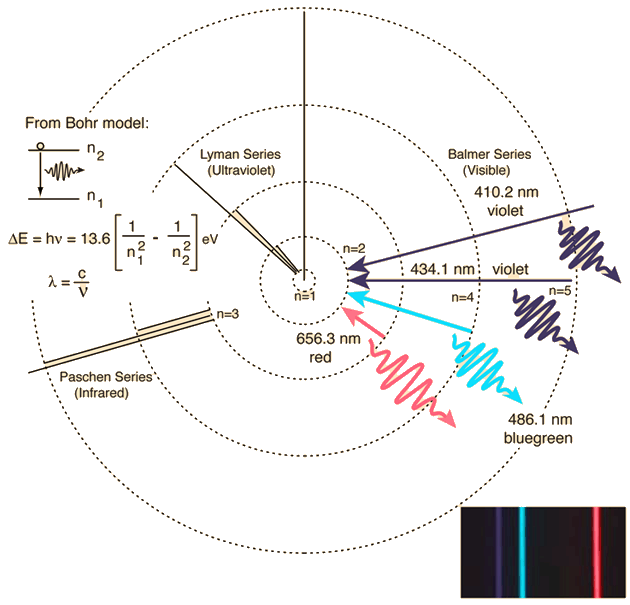
\includegraphics[width=0.65\textwidth]{figures/H.png}
\caption{\label{fig:H} Energies of order 1 electron-Volt. Our whole visual range...}
\end{figure}
\end{frame}

\begin{frame}{Voltage, Potential Energy, and Work}
Different amounts of eV:
\begin{itemize}
\item Atomic energy transitions: $\approx 1$ eV
\item X-ray energies: $\approx 1$ keV
\item Nuclear energy transitions: $\approx 1$ MeV
\item \textit{Mass of protons and neutrons}: $\approx 1$ GeV (\alert{wait, what?}...)\footnote{This is a use of Einsten's equation, $E = mc^2$.  We will return to this point later.  For another example, $m_{\rm e} = 511$ keV.}
\item \textit{Mass of other famous particles}: $\approx 100$ GeV
\item But what else is out there in nature?
\end{itemize}
\end{frame}

\begin{frame}{Voltage, Potential Energy, and Work}
\begin{figure}
\centering
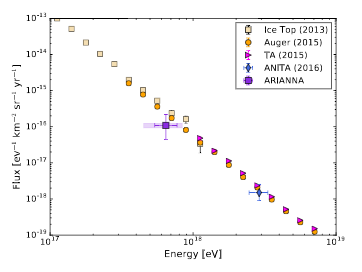
\includegraphics[width=0.6\textwidth]{figures/ARIANNA1.png}
\caption{\label{fig:arianna1} My research on the ARIANNA project has measured cosmic rays with energies of up to $10^{18}$ eV!}
\end{figure}
\end{frame}

\begin{frame}{Voltage, Potential Energy, and Work}
\begin{figure}
\centering
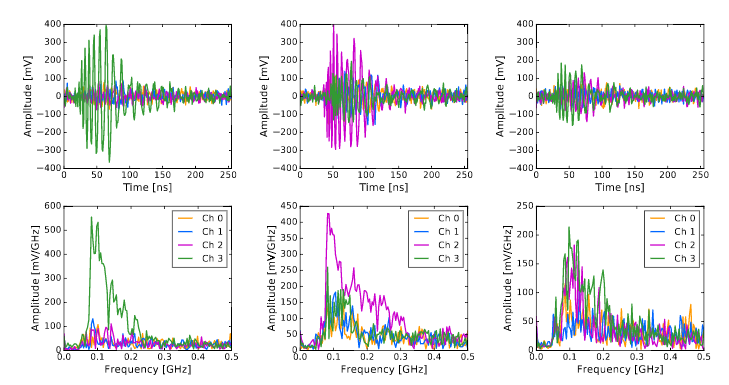
\includegraphics[width=0.6\textwidth]{figures/ARIANNA2.png}
\caption{\label{fig:arianna2} These cosmic rays (protons) have so much energy, that they make radio pulses through the atmosphere.}
\end{figure}
\end{frame}

\begin{frame}{Voltage, Potential Energy, and Work}
\begin{figure}
\centering
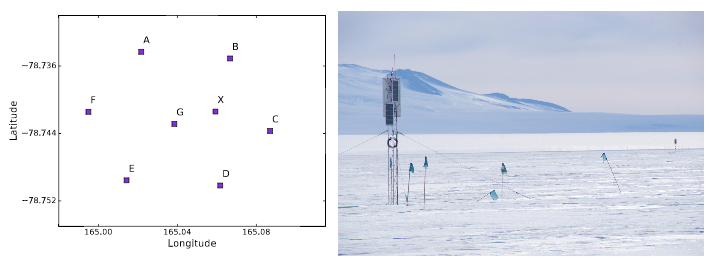
\includegraphics[width=0.6\textwidth]{figures/ARIANNA3.png}
\caption{\label{fig:arianna3} How do we do it?  We build autonomous radio detectors in the Antarctic wilderness... This would make a nice paper topic.}
\end{figure}
\end{frame}

\begin{frame}{Voltage, Potential Energy, and Work}
One electron-Volt is the energy gained by a charge of 1 electron falling through a potential of 1 Volt.
\begin{figure}
\centering
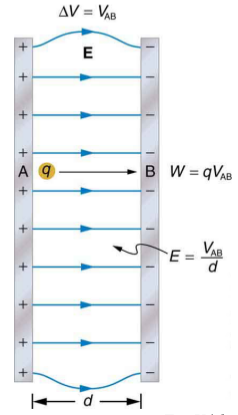
\includegraphics[width=0.25\textwidth]{figures/plates2.png}
\caption{\label{fig:plates2} Fields, voltage, and energy.}
\end{figure}
\end{frame}

\begin{frame}{Voltage, Potential Energy, and Work}
Suppose two objects have the same charge, $-e = -1.6\times 10^{-19}$ C, but one has twice the mass as the other.  If each is released through a potential of 1 V, which object gains more energy?
\begin{itemize}
\item A: The lighter one
\item B: The heavier one
\item C: They gain the same energy
\item D: Cannot determine
\end{itemize}
\end{frame}

\begin{frame}{Voltage, Potential Energy, and Work}
Suppose two objects have the same charge, $-e = -1.6\times 10^{-19}$ C, but one has twice the mass as the other.  If each is released through a potential of 1 V, which object achieves the highest speed?
\begin{itemize}
\item A: The lighter one
\item B: The heavier one
\item C: The speeds are equal because the energy is equal
\item D: Cannot determine
\end{itemize}
\end{frame}

\begin{frame}{Voltage, Potential Energy, and Work}
Consider the plates of Fig. \ref{fig:plates2}:
\begin{align}
W &= q\Delta V \\
W &= F\Delta x = qE \Delta x \\
qE \Delta x &= q\Delta V \\
E \Delta x &= \Delta V \\
E &= \frac{\Delta V}{\Delta x}
\end{align}
This derivation is good for a uniform constant field, for example, between two \textit{parallel plates of charge}.  \textbf{We proved that this field is constant back when considering charge distributions.}
\end{frame}

\begin{frame}{Voltage, Potential Energy, and Work}
So what happens if we place an electric field across two parallel plates? A charge +Q on one side and -Q on the other side develops, storing charge.  This is called a \textit{capacitor}.
\begin{figure}
\centering
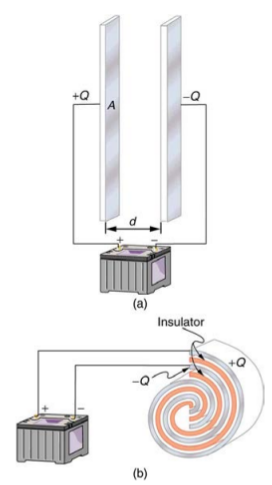
\includegraphics[width=0.25\textwidth]{figures/batt.png}
\caption{\label{fig:batt} A battery is like a parallel plate \textit{capacitor}.}
\end{figure}
\end{frame}

\section{Capacitance}

\begin{frame}{Capacitance}
What voltage is required to store $Q$? Let $\Delta V$ be the voltage difference, $E$ be the electric field strength, and $\Delta x$ be the voltage between the plates.  We already know that
\begin{equation}
\Delta V = E\Delta x
\end{equation}
\textit{But we also know from Coulomb's Law that}
\begin{equation}
E = \frac{\sigma}{\epsilon_0} = \frac{Q}{\epsilon_0 A}
\end{equation}
So we have
\begin{align}
\Delta V &= \frac{Q}{\epsilon_0 A}\Delta x \\
Q &= \left( \frac{\epsilon_0 A}{\Delta x} \right) \Delta V
\end{align}
So now we know how much charge to expect for a given voltage.  The term in parentheses is called \textit{the capacitance, C.}
\end{frame}

\begin{frame}{Capacitance}
Let the capacitor have an area $A$, and plate separation $d$.  The capacitance is
\begin{equation}
\boxed{
C = \frac{\epsilon_0 A}{d}}
\end{equation}
\textit{Capacitance} epresents the ability to store charge.  The unit of capacitance is \textbf{the farad}, after Michael Faraday (encounter mid-semester).  Scaling problems in a moment...
\end{frame}

\section{PhET Activity: Capacitor Basics}

\begin{frame}
\small
Go to the activity: \\ \vspace{0.5cm}
\url{https://phet.colorado.edu/en/simulation/capacitor-lab-basics}
\begin{enumerate}
\item Under the capacitance tab, you will find a capacitor being charged with a battery.
\item Charge the capacitor under different conditions: $d=10$ mm, $d=2$ mm, $A=100$ mm$^2$, $A=400$ mm$^2$.
\item The \textbf{voltmeter} at right is the yellow and black tool.  It allows the measurement of voltage between two points.  Measure the battery voltage and the capacitor voltage.  Why are they equal?
\item What is the charge stored for $d=2$ mm, and $A=400$ mm$^2$?
\item The light bulb tab in the bottom center contains a circuit that operates a light bulb with the energy stored in the capacitor.  Measure the voltage across the lightbulb as it is powered with the capacitor.  Sketch the voltage as a function of time.
\end{enumerate}
\end{frame}

\begin{frame}{Capacitance}
Two batteries store the same charge.  One only needs half the voltage, though.  What is true of the capacitance of the battery with the lower voltage?
\begin{itemize}
\item A: It has half the capacitance
\item B: It has the same capacitance but more charges.
\item C: It has twice the capacitance
\item D: It has half the energy
\end{itemize}
\end{frame}

\begin{frame}{Capacitance}
Two batteries have the same capacitance.  Battery 1 has half the area $A$ as battery 2.  Which of the following is true of battery 2?
\begin{itemize}
\item A: The plates are half the distance ($\Delta x$) apart
\item B: The plates are twice the distance ($\Delta x$) apart
\item C: The plates have half the voltage
\item D: The plates have twice the voltage
\end{itemize}
\end{frame}

\section{PhET Activity: Capacitor Lab}

\begin{frame}{PhET Activity: Capacitor Lab}
Similar to \textit{Capacitor basics} activity: \\ \vspace{0.5cm}
\url{https://phet.colorado.edu/en/simulation/capacitor-lab} \\ \vspace{0.5cm}
\textbf{What is the relationship between total capacitance and individual capacitances?}
\begin{enumerate}
\item How do capacitors add \textit{in series}?
\item How do capacitors add \textit{in parallel}?
\end{enumerate}
\end{frame}

\section{Capacitance and Dielectrics}

\begin{frame}{Capacitance and Dielectrics}
\begin{figure}
\centering
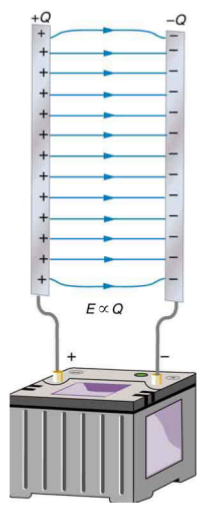
\includegraphics[width=0.25\textwidth]{figures/batt2.png}
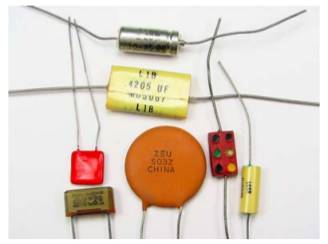
\includegraphics[width=0.5\textwidth]{figures/batt3.png}
\caption{\label{fig:batt2} A battery and a capacitor are not quite the same thing.}
\end{figure}
\end{frame}

\begin{frame}{Capacitance}
Parallel plate capacitor:
\begin{equation}
\boxed{
Q = \Delta V \left(\epsilon_0 \frac{A}{\Delta x}\right) = C\Delta V}
\end{equation}
How can we boost the charge?  Can we increase that $\epsilon_0$?  (It's a small number: $8.85 \times 10^{-12}$ N$^{-1}$ C$^2$ m$^{-2}$).  It turns out that by stuffing some insulating material between the plates \textit{boosts the capacitance...}
\end{frame}

\begin{frame}{Capacitance and Dielectrics}
Because \textit{dielectric} material reduces the field between the plates for the same charge, the voltage corresponding to that charge is reduced.  But that means \textit{higher capacitance}.
\begin{figure}
\centering
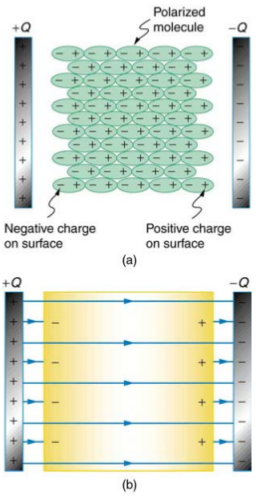
\includegraphics[width=0.25\textwidth]{figures/polar.png}
\caption{\label{fig:polar} Polarized dielectric.}
\end{figure}
\end{frame}

\begin{frame}{Capacitance and Dielectrics}
\begin{figure}
\centering
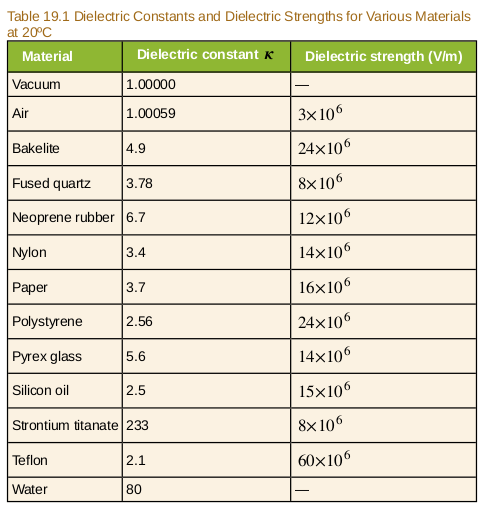
\includegraphics[width=0.5\textwidth]{figures/tableK.png}
\caption{\label{fig:tab} The middle column is the number by which $\epsilon_0$ is scaled up when dielectric is introduced.  We can't play this game indefinitely, because materials have a maximum electric field (third column) they can handle before they're ripped apart.}
\end{figure}
\end{frame}

\begin{frame}{Capacitance and Dielectrics}
\textbf{Group board exercise:} Suppose a capacitor (parallel plate) has area $A = 1$ cm$^2$ and separation $d = 1$ mm.  Using $\epsilon_0 = 8.85 \times 10^{-12}$ C$^2$ N$^{-1}$ m$^{-2}$, calculate the capacitance.  How much charge will be stored if we place 9 V across the capacitor?
\end{frame}

\begin{frame}{Capacitance and Dielectrics}
\textbf{Group board exercise:} Suppose we fill the capacitor with Teflon (see Tab. \ref{fig:tab}).  How much charge can we store with 9 V?
\end{frame}

\begin{frame}{Capacitance and Dielectrics}
\begin{figure}
\centering
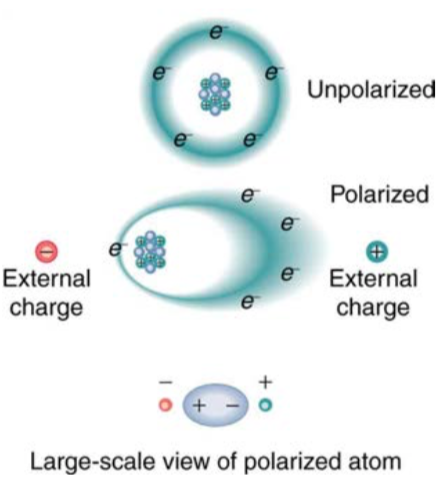
\includegraphics[width=0.5\textwidth]{figures/polar2.png}
\caption{\label{fig:polar2} Taking advantage of atomic structure in the dielectric.}
\end{figure}
\end{frame}

\begin{frame}{Capacitance and Dielectrics}
\begin{figure}
\centering
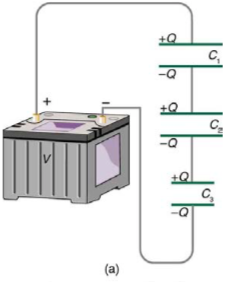
\includegraphics[width=0.4\textwidth]{figures/cap1.png} \hspace{0.2cm}
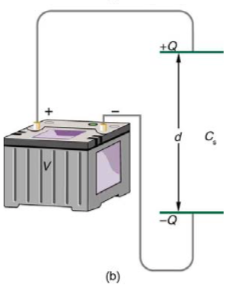
\includegraphics[width=0.4\textwidth]{figures/cap2.png}
\caption{\label{fig:cap} How do we compute the total capacitance of (a) such that we know the charge stored for a given voltage in (b)?}
\end{figure}
\end{frame}

\begin{frame}{Capacitance and Dielectrics}
\begin{itemize}
\item Notice that \textit{charge is conserved}, so $Q$ has to be the same on all capacitors
\item But that means the \textit{voltage} on the different capacitors has to obey
\begin{equation}
V = V_1 + V_2 + V_3
\end{equation}
and
\begin{align}
Q &= C_1 V_1 \\
Q &= C_2 V_2 \\
Q &= C_3 V_3
\end{align}
\end{itemize}
\end{frame}

\begin{frame}{Capacitance and Dielectrics}
\begin{itemize}
\item Combining equations:
\begin{align}
V &= \frac{Q}{C_{\rm total}} = \frac{Q}{C_1}+\frac{Q}{C_2}+\frac{Q}{C_3} \\
\frac{1}{C_{\rm total}} &= \frac{1}{C_1}+\frac{1}{C_2}+\frac{1}{C_3}
\end{align}
\item This is the capacitance for capacitors connected \textbf{in series}.
\end{itemize}
\end{frame}

\begin{frame}{Capacitance and Dielectrics}
\begin{figure}
\centering
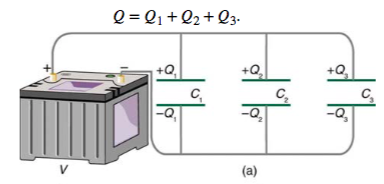
\includegraphics[width=0.4\textwidth]{figures/cap3.png} \hspace{0.2cm}
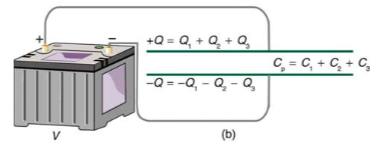
\includegraphics[width=0.4\textwidth]{figures/cap4.png}
\caption{\label{fig:cap2} How do we compute the total capacitance of (a) such that we know the charge stored for a given voltage in (b)?}
\end{figure}
\end{frame}

\begin{frame}{Capacitance and Dielectrics}
The result is:
\begin{equation}
C_{\rm total} = C_1+C_2+C_3
\end{equation}
This is the capacitance for capacitors connected \textbf{in parallel}.
\end{frame}

\begin{frame}{Capacitance and Dielectrics}
Suppose a circuit has two identical capacitors connected \textbf{in parallel}.  If a voltage of 9V stores $9 \times 10^{-6}$ C or $9\mu$C of charge, how much charge would be stored if we add two more of these same capacitors in parallel to the circuit?
\begin{itemize}
\item A: 9 $\mu$C
\item B: 4.5 $\mu$C
\item C: 18 $\mu$C
\item D: 32 $\mu$C
\end{itemize}
\end{frame}

\begin{frame}{Capacitance and Dielectrics}
Suppose we have a circuit where two capacitors are connected \textbf{in series}, and each has a \textit{capacitance} of $2\mu$F (a microfarad).  What is the total capacitance?
\begin{itemize}
\item A: $1\mu$F
\item B: $2\mu$F
\item C: $4\mu$F
\item D: $8\mu$F
\end{itemize}
\end{frame}

\begin{frame}{Capacitance and Dielectrics}
Why is the capacitance reduced by adding another capacitor?  What physically is occurring to reduce capacitance?
\begin{itemize}
\item A: It's as if the cross-sectional area is being decreased.
\item B: It's as if the plate separation is being increased.
\item C: It's as if the dielectric constant is being reduced.
\item D: It's as if the plate separation is being decreased.
\end{itemize}
\end{frame}

\section{Conclusion}

\begin{frame}{Unit 1 Summary}
\textbf{Reading: Chapters 18 and 19}
\begin{enumerate}
\item Charge, mass, the Coulomb force, and the gravitational force
\item Force fields
\item Electric potential and capacitance
\end{enumerate}
\end{frame}

\section{Answers}

\begin{frame}{Answers}
\small
\begin{columns}[T]
\begin{column}{0.5\textwidth}
\begin{itemize}
\item +1
\item The negative charges in the conductor move toward the positive charges in the rod.
\item The charges in the conductor all remain in place, and the force is attractive.
\item Both charges move, and the force on one is equal to the force on the other.
\item 45 deg
\item Symmetry...or blind luck :-)
\item The angle with respect to the x-axis is less than 45 degrees
\item B and C
\item A, B, and C
\item The field is constant.
\item $\frac{\sigma}{\epsilon_0}$
\item 0
\end{itemize}
\end{column}
\begin{column}{0.5\textwidth}
\begin{itemize}
\item $U = mgh$
\item $-mg$
\item 60 kJ and 720 kJ, respectively
\item About 7 hours
\item About 10 kJ
\item About 6 minutes
\item 9 V
\item 1 V
\item They gain the same energy
\item The lighter one
\item It has twice the capacitance
\item The plates are half the distance ($\Delta x$) apart
\end{itemize}
\end{column}
\end{columns}
\end{frame}

\end{document}
